\chapter{Knot selection in compartmental spline models: osteoarthritis of the knee}
\label{applications-con_fit_splines}

Modeled with splines, age-specific hazards are sensitive to the number and location of knots in sparse and noisy data.  The compartmental model fulfills a logical requirement of internal consistency; therefore modeling decisions for one parameter affect all epidemiological parameter estimates as seen in the following example of osteoarthritis of the knee.

Osteoarthritis (OA) is joint disorder that affects joint cartilage and underlying bone.  OA causes pain in the joints and limits movement.  Osteoarthritis of the knee is common and it causes significant morbidity, particularly in the elderly. \cite{felson_epidemiology_1988, felson_incidence_1995}  Systematic review yielded 602 rows of data representing 27 countries in 10 regions.

Since OA knee is so rare in young adults, expert priors inform the model that the onset of the disease starts at age 30.  The number and location of knots in the incidence rate between the ages 30 and 36 determine critical features of the model and may produce unexpected results as seen in Figure \ref{fig:app-oa knee knots}.

    \begin{figure}[h]
        \begin{center}
            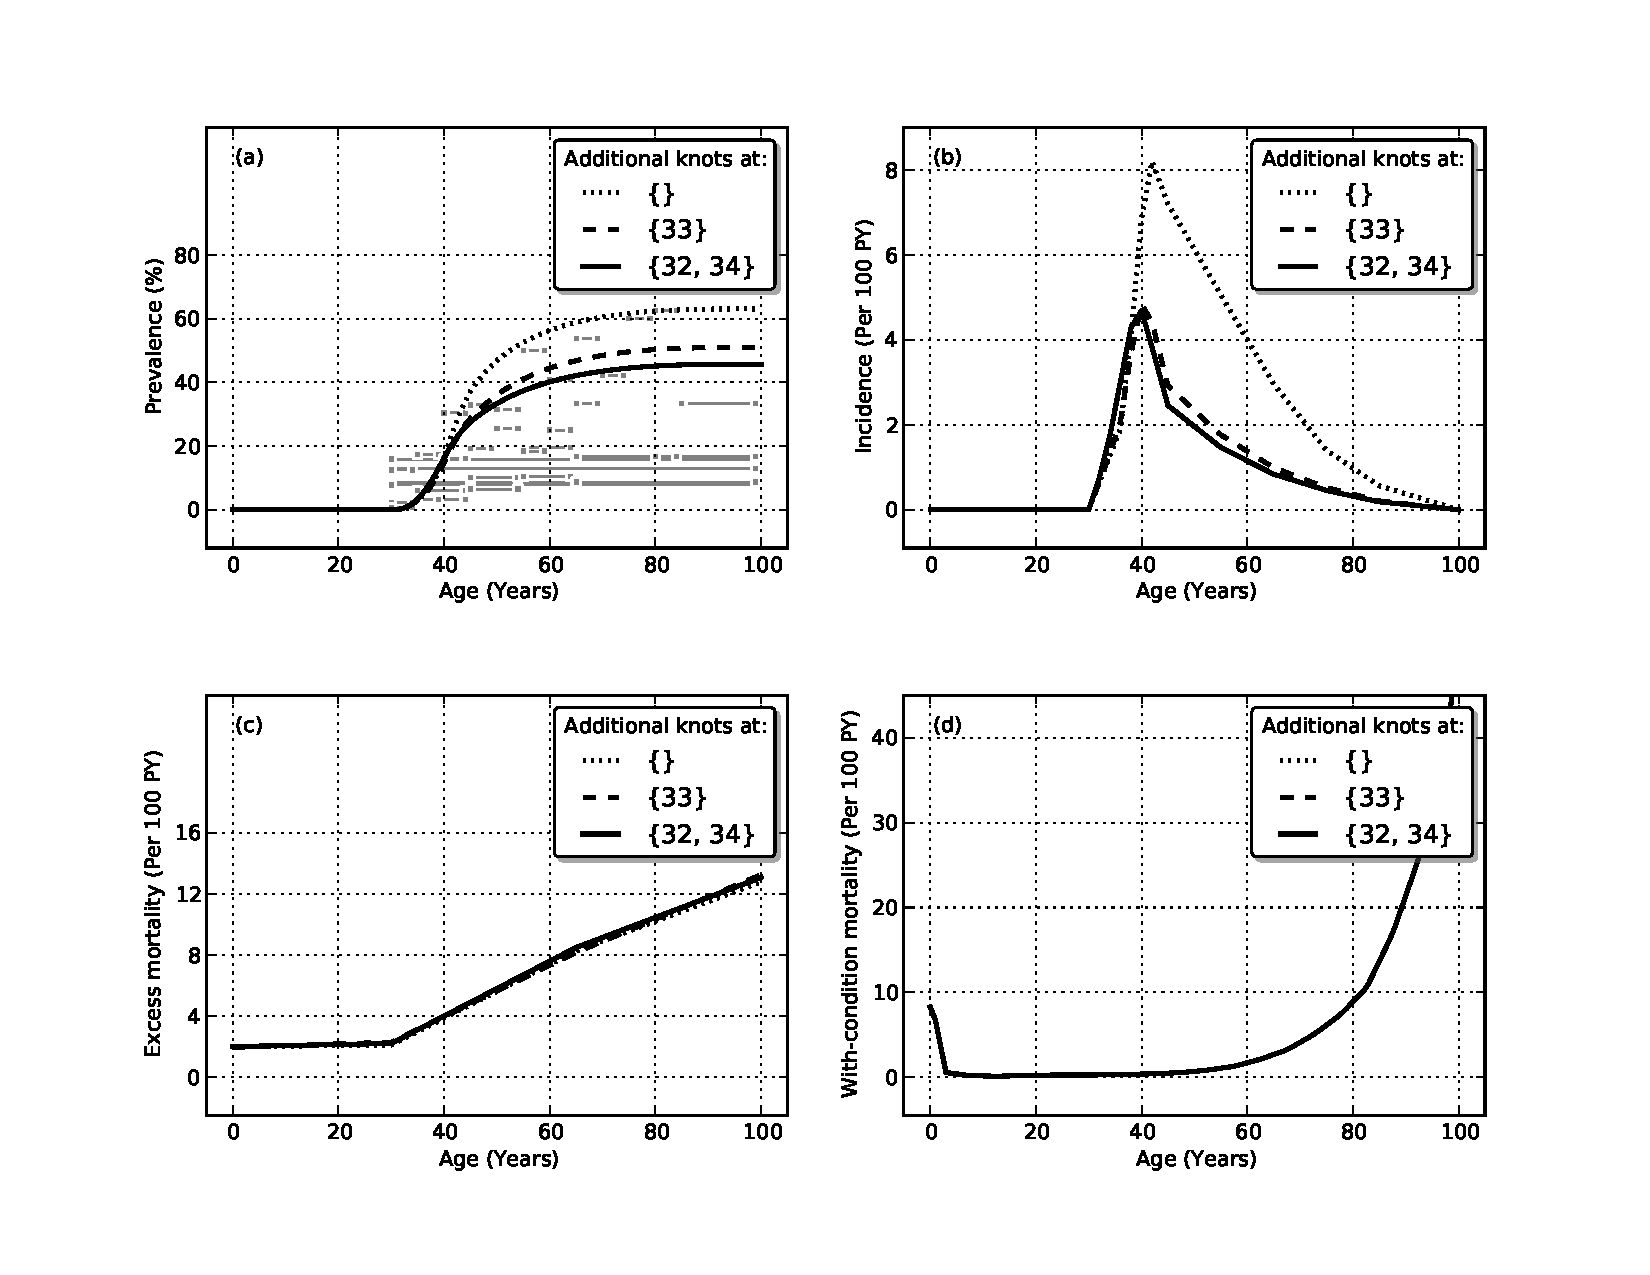
\includegraphics[width=\textwidth]{oa_knee-knots.pdf}
            \caption{Knot selection between the ages of 30 and 99 plays an important role in the estimates of OA knee epidemiologic parameters.  Prevalence estimates appear in panel (a) and incidence in panel (b) for females in South Asia with osteoarthritis of the knee in 2005.  The incidence rate of all models has knots at \{0, 30, 36, 38, 40, 42, 45, 55, 65, 75, 85, 100\}.  Between the ages of 30 and 36, the two knots, one knot and no knots models have knots at \{32, 34\}, \{33\} and \{\} respectively.}
            \label{fig:app-oa knee knots}
        \end{center}
    \end{figure}

The model is also sensitive to assumptions about the epidemiologic profile, expressed in the model as expert priors.  Figure \ref{fig:app-oa knee priors} compares assumptions about OA knee incidence.  A prior that requires zero incidence at ages greater than 99 implies that incidence decreases with age.  In other words, after a certain age, if OA knee hasn't developed, it is unlikely it ever will. Without this prior, incidence increases with age.  The logic requirement of internal consistency in the compartmental model means that prevalence estimates are also affected as shown in Figure \ref{fig:app-oa knee priors}.

    \begin{figure}[h]
        \begin{center}
            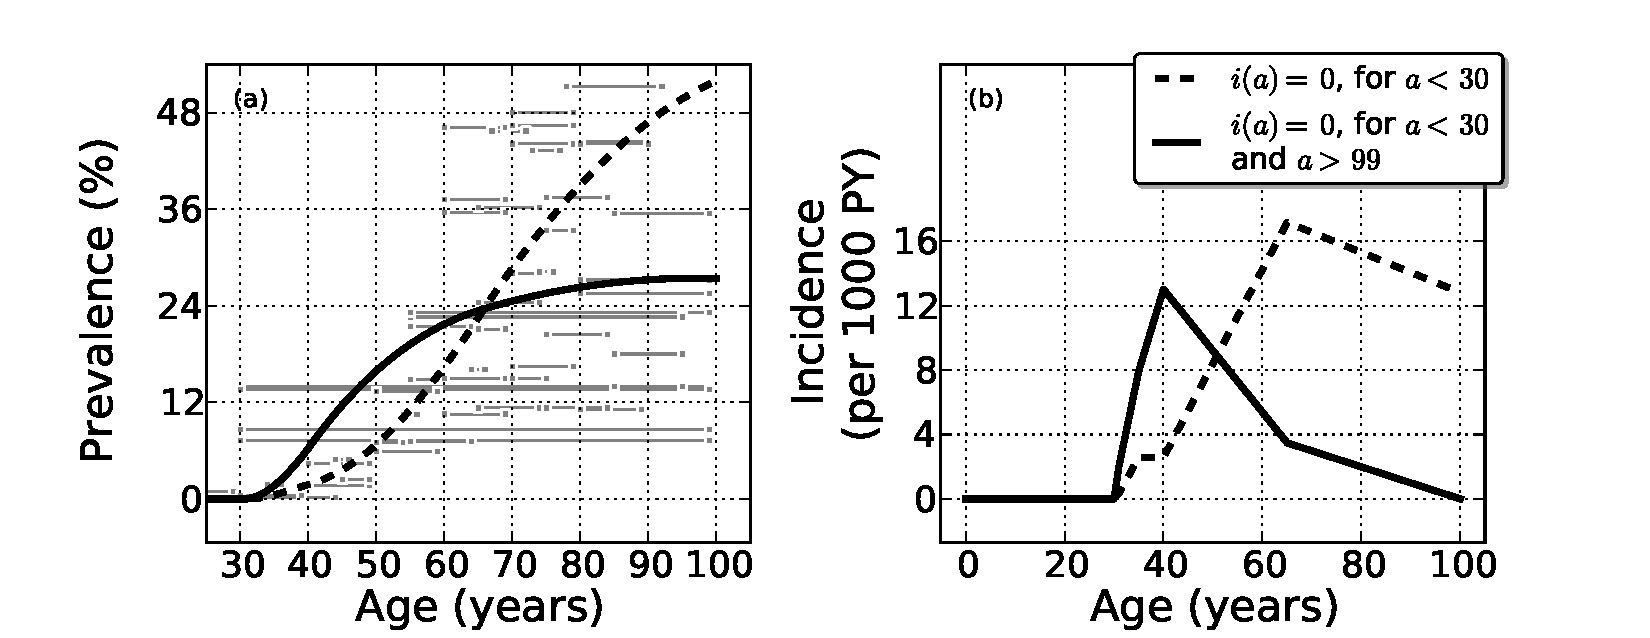
\includegraphics[width=\textwidth]{oa_knee-i_prior.pdf}
            \caption{A comparison of compartmental models with and without a prior stipulating no onset of the disease in ages greater than 99.  Prevalence (panel (a)) and incidence (panel (b)) estimates for South Asian females with OA knee in 2005.}
            \label{fig:app-oa knee priors}
        \end{center}
    \end{figure} 